\section{Motivation} 
\label{sec:int_motivation} 
 
 
With the recent technological advancements, smartphones are now capable of carrying a wide variety of sensors. This opportunity, in addition to its wide utilisation, made smartphones a perfect candidate for indoor location systems. Therefore, systems that make use of technologies that are compatible with smartphones, are capable of taking advantage of them, removing the need of having system-specific devices. 
 
Currently the attention is focused on the improvement and creation of new means to achieve better positioning results, as it is possible to notice from the vast number of existing methods and algorithms available to infer someone's location. Although this part is of great importance, as the success of a location system in the present day is highly dependent on its accuracy levels, another relevant concern for any system is their energetic consumption.

With smartphones being heavily used by any modern system, it is fundamental to comprehend that they are personal devices with a limited amount of resources. The most relevant resource is the battery, a constraint that can't be entirely taken by the system.  
 
Another important factor is that an indoor system needs to be scalable, with respect to the number of users in the same indoor building or in terms of being capable of working with different deployments/buildings. Systems created with the purpose of being used in different environments need to provide an architecture capable of working seamlessly when moving between buildings. As such it is required that the smartphone (mobile agent) is capable of obtaining its own location wherever the system is deployed.   
 
Since we live in an era dominated by smartphones, their evolution has allowed for developing systems which rely on its sensors and processing capacities to present a solution which isn't dependant on specific hardware. The first condition that is imposed onto the systems is the compatibility with smartphones, i.e. the required sensors needs to exist on the generic hardware of smartphones. Once this barrier is surpassed, these generic systems are immediately faced with three fundamental decisions which will define the architecture of the system and which can be seen on figure \ref{fig:choices}. 
 
\begin{figure}[htp] 
\centering 
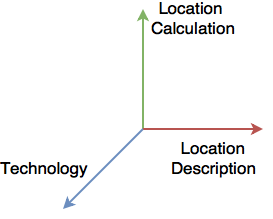
\includegraphics[width=0.5\linewidth]{1.Chapter/vectors.png} 
\caption[Three fundamental choices in Indoor systems]{Three fundamental choices in Indoor systems} 
\label{fig:choices} 
\end{figure} 

The first decision, Technology, defines the technology which is to be used in conjunction with the smartphone and consequently the way that location data is to be collected. There is a wide range of possibilities for this choice, be it BLE beacons, Wi-Fi Access points, LED lamps or just the microphone for sound collection, and each has an impact on the way that the system functions and on its performance.  
 
 
The second question is the location algorithm, which fundamentally depends on the target requirements of the system, if it's required to provide accurate location of a user or if a more descriptive location, such as indicating the room in which the user is located, is enough. There is already a great number of different usable algorithms for each indoor capable technology. Therefore, the choice depends on the way that distance calculation is obtained, be it through time or signal strength, and obviously the technology. 
 
 
The third and last question is about which way the location will be described. When dealing with outdoor location systems, the provided location is always characterised by four values: latitude, longitude, altitude and datum. In indoor systems, the surrounding environment can be of many shapes and as such different ways of representing location are necessary. If one thinks about providing indoor location in an office, the precise location isn't as relevant as just knowing the general location, i.e. a building specific description of the location in the form of building, floor and room. On other environments such as supermarkets or even in the previous example, where the objective is to provide a more precise location description, a cartesian coordinate system (x,y) is required. 
 